\documentclass[12pt]{article}

% Opening
\title{Applied Combinatorics Homework 4}
\author{Akash Narayanan}
\usepackage{amsmath, amsfonts, amssymb, amsthm, enumitem, tikz}
\usepackage{caption, subcaption, float}

% Problem counters
\newcounter{chapternumber}


% Problem environment
\theoremstyle{definition}
\newtheorem{problem-internal}{Problem}[chapternumber]
\newenvironment{problem}{
  \medskip
  \begin{problem-internal}
}{
\end{problem-internal}
}

% Solution environment
\newenvironment{solution}{
  \begin{proof}[Solution]
    \vspace{-8px}
    \setlength{\parskip}{4px}
    \setlength{\parindent}{0px}
}{
\end{proof}
}

% Theorem environment
\newtheorem*{theorem}{Theorem}

\begin{document}

  \maketitle

  % Problem 6.11
  \setcounter{chapternumber}{6}
  \setcounter{problem-internal}{10}
  \begin{problem}
    A restaurant chef has designed a new set of dishes for his menu.
    His set of dishes contains 10 main courses, and he will select a subset of them to place on the menu each night.
    To ensure variety of main courses for his patrons, he wants to guarantee that a night's menu is neither completely contained in nor completely contains another night's menu.
    What is the largest number of menus he can plan using his 10 main courses subject to this requirement?
  \end{problem}

  \begin{solution}
    Consider the subset lattice on 10 elements, where \(A \leq B\) when \(A \subseteq B\).
    Then every subset can be considered a menu and the chef wants to ensure that no two menus contain one another.
    Thus, the problem is equivalent to finding the width of this poset.
    By Sperner's Theorem, the width of the subset lattice on \(t\) elements is \(C\left(t, \lfloor{\frac{t}{2}}\rfloor\right)\).
    Thus, the width of the poset in consideration is \(C\left(10, 5\right) = 252\).
    That is, the largest number of menus he can plan is 252.
  \end{solution}

  % Problem 6.14
  \setcounter{problem-internal}{13}
  \begin{problem}
    Find an interval representation for the poset shown below, or give a reason why one does not exist.

    \begin{figure}[H]
      \centering
      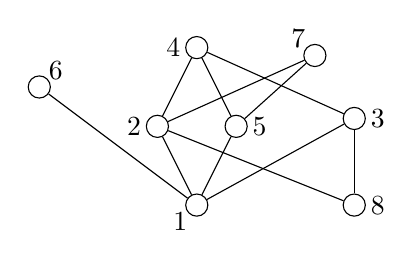
\begin{tikzpicture}
        [scale=1,every node/.style={draw,shape=circle,fill=white,inner sep=0,minimum size=8pt}, every draw/.style={line width=0.25mm, black}]

        \node[label=225:{1}] (v1) at (0, 0) {};
        \node[label=180:{2}] (v2) at (-0.5, 1) {};
        \node[label=0:{3}] (v3) at (2, 1.1) {};
        \node[label=180:{4}] (v4) at (0, 2) {};
        \node[label=0:{5}] (v5) at (0.5, 1) {};
        \node[label=45:{6}] (v6) at (-2, 1.5) {};
        \node[label=135:{7}] (v7) at (1.5, 1.9) {};
        \node[label=0:{8}] (v8) at (2, 0) {};

        \draw (v1) -- (v2);
        \draw (v1) -- (v3);
        \draw (v1) -- (v5);
        \draw (v1) -- (v6);
        \draw (v2) -- (v4);
        \draw (v2) -- (v7);
        \draw (v2) -- (v8);
        \draw (v3) -- (v4);
        \draw (v3) -- (v8);
        \draw (v4) -- (v5);
        \draw (v5) -- (v7);

      \end{tikzpicture}
    \end{figure}
  \end{problem}

  \begin{solution}
    We start by listing each element's down set and up set.
    Recall that \(D \left( x \right) = \{y \in \textbf{P} \mid y < x \text{ in } \textbf{P}\}\) and \(U \left( x \right) = \{y \in \textbf{P} \mid y > x \text{ in } \textbf{P}\}\).
    \begin{align*}
      D \left( 1 \right) &= \emptyset & U \left( 1 \right) &= \{2, 3, 4, 5, 6, 7\} \\
      D \left( 2 \right) &= \{1, 8\} & U \left( 2 \right) &= \{4, 7\} \\
      D \left( 3 \right) &= \{1, 8\} & U \left( 3 \right) &= \{4\} \\
      D \left( 4 \right) &= \{1, 2, 3, 5, 8\} & U \left( 4 \right) &= \emptyset \\
      D \left( 5 \right) &= \{1\} & U \left( 5 \right) &= \{4, 7\} \\
      D \left( 6 \right) &= \{1\} & U \left( 6 \right) &= \emptyset \\
      D \left( 7 \right) &= \{1, 2, 5, 8\} & U \left( 7 \right) &= \emptyset \\
      D \left( 8 \right) &= \emptyset & U \left( 8 \right) &= \{2, 3, 4, 5, 7\}
    \end{align*}
    Note that every down set is comparable by inclusion, so there is an interval representation for the poset shown.
    We rank the down sets from smallest to largest and the up sets from largest to smallest, with the rankings listed to the right of the set.
    The rankings define the function \(I\left( x \right)\) mapping each element of the poset to the intervals shown below.
    \begin{align*}
      I\left( 1 \right) &= [1, 1] \\
      I\left( 2 \right) &= [3, 3] \\
      I\left( 3 \right) &= [3, 4] \\
      I\left( 4 \right) &= [5, 5] \\
      I\left( 5 \right) &= [2, 3] \\
      I\left( 6 \right) &= [2, 5] \\
      I\left( 7 \right) &= [4, 5] \\
      I\left( 8 \right) &= [1, 4]
    \end{align*}
    The corresponding interval graph is shown below.
    \begin{figure}[H]
      \centering
      \begin{tikzpicture}

        \draw (1, 0.00) -- node[above] {1} (1, 0.00);
        \draw (3, 0.00) -- node[above] {2} (3, 0.00);
        \draw (3, 0.75) -- node[above] {3} (4, 0.75);
        \draw (5, 0.00) -- node[above] {4} (5, 0.00);
        \draw (2, 1.50) -- node[above] {5} (3, 1.50);
        \draw (2, 2.25) -- node[above] {6} (5, 2.25);
        \draw (4, 1.50) -- node[above] {7} (5, 1.50);
        \draw (1, 3.00) -- node[above] {8} (4, 3.00);

        \fill (1, 0.00) circle (0.1);
        \fill (3, 0.00) circle (0.1);
        \fill (3, 0.75) circle (0.1); \fill (4, 0.75) circle (0.1);
        \fill (5, 0.00) circle (0.1);
        \fill (2, 1.50) circle (0.1); \fill (3, 1.50) circle (0.1);
        \fill (2, 2.25) circle (0.1); \fill (5, 2.25) circle (0.1);
        \fill (4, 1.50) circle (0.1); \fill (5, 1.50) circle (0.1);
        \fill (1, 3.00) circle (0.1); \fill (4, 3.00) circle (0.1);

        \draw (-1.5, -1) -- (6.5, -1);

        \node[label=below:{-1}] at (-1, -1) {};
        \node[label=below:{0}] at (0, -1) {};
        \node[label=below:{1}] at (1, -1) {};
        \node[label=below:{2}] at (2, -1) {};
        \node[label=below:{3}] at (3, -1) {};
        \node[label=below:{4}] at (4, -1) {};
        \node[label=below:{5}] at (5, -1) {};
        \node[label=below:{6}] at (6, -1) {};

      \end{tikzpicture}
    \end{figure}
  \end{solution}

  % Problem 6.15
  \begin{problem}
    Find an interval representation for the poset shown below, or give a reason why one does not exist.

    \begin{figure}[H]
      \centering
      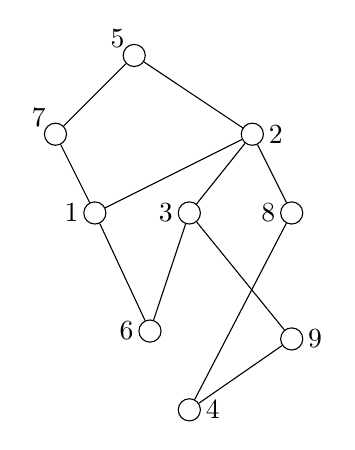
\begin{tikzpicture}
        [scale=1,every node/.style={draw,shape=circle,fill=white,inner sep=0,minimum size=8pt}, every draw/.style={line width=0.25mm, black}]

        \node[label=180:{1}] (v1) at (0, 0) {};
        \node[label=0:{2}] (v2) at (2, 1) {};
        \node[label=180:{3}] (v3) at (1.2 , 0) {};
        \node[label=0:{4}] (v4) at (1.2, -2.5) {};
        \node[label=135:{5}] (v5) at (0.5, 2) {};
        \node[label=180:{6}] (v6) at (0.7, -1.5) {};
        \node[label=135:{7}] (v7) at (-0.5, 1) {};
        \node[label=180:{8}] (v8) at (2.5, 0) {};
        \node[label=0:{9}] (v9) at (2.5, -1.6) {};

        \draw (v1) -- (v2);
        \draw (v1) -- (v6);
        \draw (v1) -- (v7);
        \draw (v2) -- (v3);
        \draw (v2) -- (v5);
        \draw (v2) -- (v8);
        \draw (v3) -- (v6);
        \draw (v3) -- (v9);
        \draw (v4) -- (v8);
        \draw (v4) -- (v9);
        \draw (v5) -- (v7);

      \end{tikzpicture}
    \end{figure}
  \end{problem}

  \begin{solution}
    We start by listing each element's down set and up set.
    \begin{align*}
      D \left( 1 \right) &= \{6\} & U \left( 1 \right) &= \{2, 5, 7\} \\
      D \left( 2 \right) &= \{1, 3, 4, 6, 8, 9\} & U \left( 2 \right) &= \{5\} \\
      D \left( 3 \right) &= \{4, 6, 9\} & U \left( 3 \right) &= \{2, 5\} \\
      D \left( 4 \right) &= \emptyset & U \left( 4 \right) &= \{2, 3, 5, 8, 9\} \\
      D \left( 5 \right) &= \{1, 2, 3, 4, 6, 7, 8, 9\} & U \left( 5 \right) &= \emptyset \\
      D \left( 6 \right) &= \emptyset & U \left( 6 \right) &= \{1, 2, 3, 5, 7\} \\
      D \left( 7 \right) &= \{1, 6\} & U \left( 7 \right) &= \{5\} \\
      D \left( 8 \right) &= \{4\} & U \left( 8 \right) &= \{2, 5\}
    \end{align*}
    Notice that \(D \left( 1 \right)\) and \(D \left( 8 \right)\) are not comparable by inclusion.
    Then the four elements \(\{1, 6, 4, 8\}\) form a \(2 + 2\).
    By Fishburn's Theorem, the poset is not an interval order.
  \end{solution}

  % Problem 6.17
  \setcounter{problem-internal}{16}
  \begin{problem}
    Find an interval representation for the poset shown below, or give a reason why one does not exist.

    \begin{figure}[H]
      \centering
      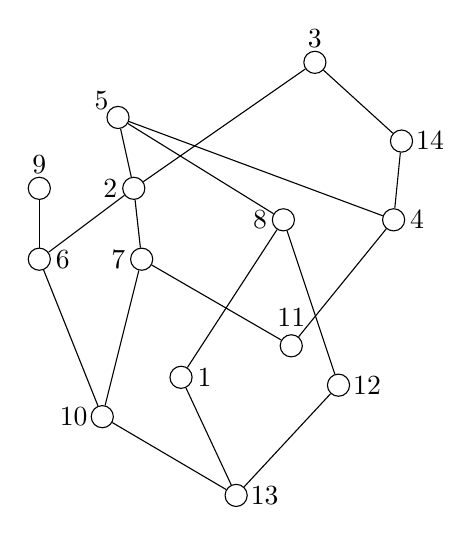
\begin{tikzpicture}
        [scale=1,every node/.style={draw,shape=circle,fill=white,inner sep=0,minimum size=8pt}, every draw/.style={line width=0.25mm, black}]

        \node[label=0:{1}] (v1) at (0, 0) {};
        \node[label=180:{2}] (v2) at (-0.6, 2.4) {};
        \node[label=90:{3}] (v3) at (1.7, 4) {};
        \node[label=0:{4}] (v4) at (2.7, 2) {};
        \node[label=135:{5}] (v5) at (-0.8, 3.3) {};
        \node[label=0:{6}] (v6) at (-1.8, 1.5) {};
        \node[label=180:{7}] (v7) at (-0.5, 1.5) {};
        \node[label=180:{8}] (v8) at (1.3, 2) {};
        \node[label=90:{9}] (v9) at (-1.8, 2.4) {};
        \node[label=180:{10}] (v10) at (-1, -0.5) {};
        \node[label=90:{11}] (v11) at (1.4, 0.4) {};
        \node[label=0:{12}] (v12) at (2, -0.1) {};
        \node[label=0:{13}] (v13) at (0.7, -1.5) {};
        \node[label=0:{14}] (v14) at (2.8, 3) {};

        \draw (v1) -- (v8);
        \draw (v1) -- (v13);
        \draw (v2) -- (v3);
        \draw (v2) -- (v5);
        \draw (v2) -- (v6);
        \draw (v2) -- (v7);
        \draw (v3) -- (v14);
        \draw (v4) -- (v5);
        \draw (v4) -- (v11);
        \draw (v4) -- (v14);
        \draw (v5) -- (v8);
        \draw (v6) -- (v9);
        \draw (v6) -- (v10);
        \draw (v7) -- (v10);
        \draw (v7) -- (v11);
        \draw (v8) -- (v12);
        \draw (v10) -- (v13);
        \draw (v12) -- (v13);

      \end{tikzpicture}
    \end{figure}
  \end{problem}

  \begin{solution}
    Note that \(D \left( 9 \right) = \{6, 10, 13\}\) but \(D \left( 8 \right) = \{1, 12, 13\}\).
    Since the two down sets are not comparable by incusion, we can find that the four elements \(\{6, 9, 12, 8\}\) form a \(2 + 2\).
    By Fishburn's Theorem, the poset is not an interval order.
  \end{solution}

  % Problem 6.18
  \begin{problem}
    Use the First Fit algorithm (ordering by left endpoints) to find the width \(w\) of the interval order shown below and a partition into \(w\) chains.
    Also give an antichain with \(w\) points.

    \begin{figure}[H]
      \centering
      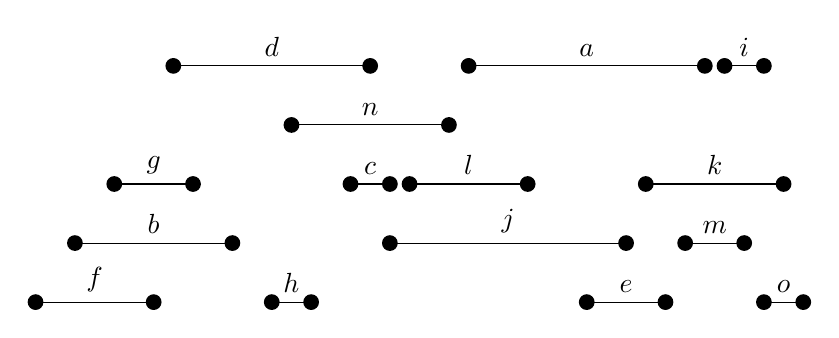
\begin{tikzpicture}

        \draw (0.5, 3) -- node[above] {\(a\)} (3.5, 3);
        \draw (-4.5, 0.75) -- node[above] {\(b\)} (-2.5, 0.75);
        \draw (-1, 1.5) -- node[above] {\(c\)} (-0.5, 1.5);
        \draw (-3.25, 3) -- node[above] {\(d\)} (-0.75, 3);
        \draw (2, 0) -- node[above] {\(e\)} (3, 0);
        \draw (-5, 0) -- node[above] {\(f\)} (-3.5, 0);
        \draw (-4, 1.5) -- node[above] {\(g\)} (-3, 1.5);
        \draw (-2, 0) -- node[above] {\(h\)} (-1.5, 0);
        \draw (3.75, 3) -- node[above] {\(i\)} (4.25, 3);
        \draw (-0.5, 0.75) -- node[above] {\(j\)} (2.5, 0.75);
        \draw (2.75, 1.5) -- node[above] {\(k\)} (4.5, 1.5);
        \draw (-0.25, 1.5) -- node[above] {\(l\)} (1.25, 1.5);
        \draw (3.25, 0.75) -- node[above] {\(m\)} (4, 0.75);
        \draw (-1.75, 2.25) -- node[above] {\(n\)} (0.25, 2.25);
        \draw (4.25, 0) -- node[above] {\(o\)} (4.75, 0);

        \fill (0.5, 3) circle (0.1); \fill (3.5, 3) circle (0.1);
        \fill (-4.5, 0.75) circle (0.1); \fill (-2.5, 0.75) circle (0.1);
        \fill (-1, 1.5) circle (0.1); \fill (-0.5, 1.5) circle (0.1);
        \fill (-3.25, 3) circle (0.1); \fill (-0.75, 3) circle (0.1);
        \fill (2, 0) circle (0.1); \fill (3, 0) circle (0.1);
        \fill (-5, 0) circle (0.1); \fill (-3.5, 0) circle (0.1);
        \fill (-4, 1.5) circle (0.1); \fill (-3, 1.5) circle (0.1);
        \fill (-2, 0) circle (0.1); \fill (-1.5, 0) circle (0.1);
        \fill (3.75, 3) circle (0.1); \fill (4.25, 3) circle (0.1);
        \fill (-0.5, 0.75) circle (0.1); \fill (2.5, 0.75) circle (0.1);
        \fill (2.75, 1.5) circle (0.1); \fill (4.5, 1.5) circle (0.1);
        \fill (-0.25, 1.5) circle (0.1); \fill (1.25, 1.5) circle (0.1);
        \fill (3.25, 0.75) circle (0.1); \fill (4, 0.75) circle (0.1);
        \fill (-1.75, 2.25) circle (0.1); \fill (0.25, 2.25) circle (0.1);
        \fill (4.25, 0) circle (0.1); \fill (4.75, 0) circle (0.1);

      \end{tikzpicture}
    \end{figure}
  \end{problem}

  \begin{solution}
    Using the first fit algorithm, the interval order is colored as shown below.
    \begin{figure}[H]
      \centering
      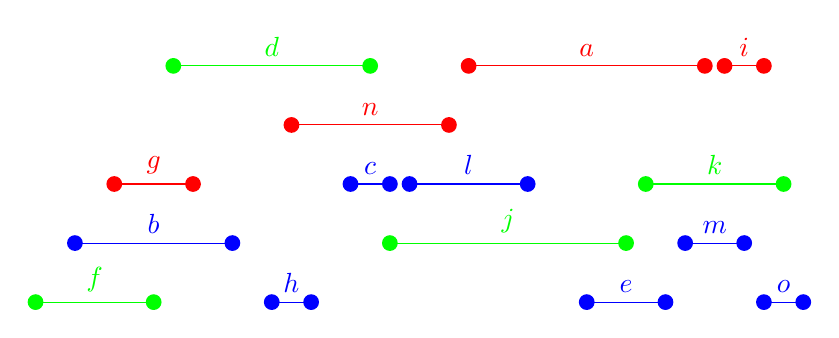
\begin{tikzpicture}

        \draw[red] (0.5, 3) -- node[above] {\(a\)} (3.5, 3);
        \draw[blue] (-4.5, 0.75) -- node[above] {\(b\)} (-2.5, 0.75);
        \draw[blue] (-1, 1.5) -- node[above] {\(c\)} (-0.5, 1.5);
        \draw[green] (-3.25, 3) -- node[above] {\(d\)} (-0.75, 3);
        \draw[blue] (2, 0) -- node[above] {\(e\)} (3, 0);
        \draw[green] (-5, 0) -- node[above] {\(f\)} (-3.5, 0);
        \draw[red] (-4, 1.5) -- node[above] {\(g\)} (-3, 1.5);
        \draw[blue] (-2, 0) -- node[above] {\(h\)} (-1.5, 0);
        \draw[red] (3.75, 3) -- node[above] {\(i\)} (4.25, 3);
        \draw[green] (-0.5, 0.75) -- node[above] {\(j\)} (2.5, 0.75);
        \draw[green] (2.75, 1.5) -- node[above] {\(k\)} (4.5, 1.5);
        \draw[blue] (-0.25, 1.5) -- node[above] {\(l\)} (1.25, 1.5);
        \draw[blue] (3.25, 0.75) -- node[above] {\(m\)} (4, 0.75);
        \draw[red] (-1.75, 2.25) -- node[above] {\(n\)} (0.25, 2.25);
        \draw[blue] (4.25, 0) -- node[above] {\(o\)} (4.75, 0);

        \fill[red] (0.5, 3) circle (0.1); \fill[red] (3.5, 3) circle (0.1);
        \fill[blue] (-4.5, 0.75) circle (0.1); \fill[blue] (-2.5, 0.75) circle (0.1);
        \fill[blue] (-1, 1.5) circle (0.1); \fill[blue] (-0.5, 1.5) circle (0.1);
        \fill[green] (-3.25, 3) circle (0.1); \fill[green] (-0.75, 3) circle (0.1);
        \fill[blue] (2, 0) circle (0.1); \fill[blue] (3, 0) circle (0.1);
        \fill[green] (-5, 0) circle (0.1); \fill[green] (-3.5, 0) circle (0.1);
        \fill[red] (-4, 1.5) circle (0.1); \fill[red] (-3, 1.5) circle (0.1);
        \fill[blue] (-2, 0) circle (0.1); \fill[blue] (-1.5, 0) circle (0.1);
        \fill[red] (3.75, 3) circle (0.1); \fill[red] (4.25, 3) circle (0.1);
        \fill[green] (-0.5, 0.75) circle (0.1); \fill[green] (2.5, 0.75) circle (0.1);
        \fill[green] (2.75, 1.5) circle (0.1); \fill[green] (4.5, 1.5) circle (0.1);
        \fill[blue] (-0.25, 1.5) circle (0.1); \fill[blue] (1.25, 1.5) circle (0.1);
        \fill[blue] (3.25, 0.75) circle (0.1); \fill[blue] (4, 0.75) circle (0.1);
        \fill[red] (-1.75, 2.25) circle (0.1); \fill[red] (0.25, 2.25) circle (0.1);
        \fill[blue] (4.25, 0) circle (0.1); \fill[blue] (4.75, 0) circle (0.1);

      \end{tikzpicture}
    \end{figure}
    The First Fit algorithm gives the chromatic number \(\chi \left( \textbf{G} \right)\) for interval graphs.
    Furthermore, for interval graphs \(\chi \left( \textbf{G} \right) = \omega \left( \textbf{G} \right)\).
    Therefore, the width of the interval order is 3.
    The interval order is partitioned into the following chains: \(\{f, d, j, k\}, \{b, h, c, l, e, m, o\}, \{g, n, a, i\}\).
    An antichain with 3 points is \(\{b, f, g\}\).
  \end{solution}

  % Problem 6.19
  \begin{problem}
    Complete the proof of the theorem shown below.
  \end{problem}

  \begin{theorem}
    If \textbf{P} is a poset excluding \(2 + 2\), then the following statements hold.
    \begin{enumerate}
      \item The number of down sets equals the number of up sets. That is, \\
      \(|\mathcal{D}| = |\mathcal{U}|\).
      \item For each \(x \in X\), if \(I \left( x \right) = [i, j]\), then \(i \leq j\) in \(\mathbb{R}\).
      \item For each \(x, y \in X\), if \(I \left(x \right) = [i, j]\) and \(I \left( y \right) = [k, l]\), then \(x < y\) in \textbf{P} if and only if \(j < k\) in \(\mathbb{R}\).
      \item The integer \(d\) is the least positive integer for which \textbf{P} has an interval representation using integer end points from \([d]\). This representation is unique.
    \end{enumerate}
  \end{theorem}

  \begin{solution}
    Recall that \(D \left( x \right) = \{y \in X \mid y < x \text{ in \textbf{P}}\}\).
    Consider the set complement \(D' \left( x \right) = \{y \in X \mid y \notin D \left( x \right) \}\).
    But \(U \left( x \right) = \{y \in X \mid y > x \text{ in \textbf{P}}\}\) so clearly \(U \left( x \right) \subseteq D' \left( x \right)\).
    Since this holds for all \(x \in X\), every up set corresponds with at least one down set.
    That is, \(| \mathcal{U} | \leq | \mathcal{D} |\).
    Similarly, \(D \left( x \right) \subseteq U' \left( x \right)\) for all \(x \in X\), so \(| \mathcal{D} | \leq | \mathcal{U} |\).
    Therefore, \(| \mathcal{U} | = | \mathcal{D} | = d\).

    Suppose now we have an ascending chain of down sets and a descending chain of up sets
    \begin{align*}
      \emptyset = D_{1} \subset D_{2} \subset D_{3} \subset \cdots \subset D_{d} \\
      U_{1} \supset U_{2} \supset U_{3} \supset \cdots \supset U_{d} = \emptyset
    \end{align*}
    We define an interval representation \(I\) of \textbf{P} by letting \(I \left( x \right) = [i, j]\) for all \(x \in X\), where \(D \left( x \right) = D_{i}\) and \(U \left( x \right) = U_{j}\).
    Let \(x \in X\). If \(D \left( x \right) = \emptyset\) then \(i = 1\) and \(j \geq i\) for any up set \(U \left( x \right)\).
    Suppose then that \(D_{i}\) is non-empty.
    Then for all \(k < i\), there exists \(y \in D_{i}\) such that \(U \left( y \right) = U_{k}\).
    But clearly \(x \in U \left( y \right)\).
    Therefore, we must have \(i \leq j\) in \(\mathbb{R}\).

    Assume that for each \(x, y \in \textbf{P}\), \(I \left( x \right) = [i, j]\) and \(I \left( y \right) = [k, l]\).
    Suppose that \(j < k\) in \(\mathbb{R}\).
    Then \(U_{j} \supset U_{k}\), but every proper superset of \(U_{k}\) contains \(y\) (as evidenced in the proof of statement 2).
    Thus, \(y \in U_{j}\) so \(y > x\).
    Now suppose that \(x < y\).
    Then \(y \in U \left( x \right) = U_{j}\).
    Furthermore, \(U_{k} = U \left( y \right)\) so \(y \notin U_{k}\).
    Then \(U_{k} \subset U_{j}\) and it follows that \(j < k\).

    Let \(i \in [d]\). We will show that there are elements \(x, y \in X\) such that \(I \left( x \right) = [a, i]\) and \(I \left( y \right) = [i, b]\).
    Certainly \(i \leq d\) so there is some \(x \in X\) for which \(U \left( x \right) = U_{i}\). That is, \(I \left( x \right) = [a, i]\).
    Similarly, there is some \(y \in X\) for which \(D \left( y \right) = U_{i}\) so \(I \left( y \right) = [i, b]\).
    Therefore, every element of \([d]\) is used as a left and right endpoint so you need at most a set of size \(d\) to create a unique interval order.
    Additionally, there are \(d\) distinct down sets, each of which serves as a left endpoint for some interval. Thus, one needs at minimum a set of size \(d\).
    In conclusion, \(d\) is the smallest integer such that \textbf{P} has a unique interval representation using integer end points from \([d]\).

  \end{solution}

\end{document}
